\chapter{Introduction}
\label{introduction}
In this chapter the working environment, project background and all involved companies will be introduced. Furthermore, the aim and limitations of the project will be explained.

%% Section 1 %%
\section{Working environment}

\subsection{Sweden \& Halmstad}
Sweden is part of Scandinavia and located in Northern Europe. It has a population of around 10 million people from which 85\% are living in cities. Sweden is part of the European Union but has retained its own currency Swedish krona (SEK). The largest and at the same time capital city of Sweden is Stockholm with about 930.000 citizens.\\

Halmstad is currently the $19^{th}$ biggest city of Sweden. It is located in the region Halland, between the two cities Malmö and Gothenburg on the west-coast of Sweden. Halmstad has around 94.000 inhabitants and is widely known as one of Sweden's biggest tourist destinations. Further the big port of Halmstad allows for an economical and industrial development of the city. Tourism, trade, industry and education are the biggest employment sectors in Halmstad.\cite{Halmstad} 

\subsection{Halmstad University}
The University of Halmstad was founded in 1970. In 1973, as a pilot project, the pre-school teacher education course was established. In 1983 Halmstad University was formally inaugurated as an independent University and in 1988 the University moved to Larsfrid in the eastern part of Halmstad, where it is located today.
To the date of 21.02.2020 Halmstad University employs 607 employees, including 49 professors, 82 Ph.D students, 13 Doctoral degrees and 5 Licentiate degrees. It has a total of 11.411 students, including 5.491 full time students. Further the University takes active part in the development of society, by collaborating with both the private and the public sector in a wide variety of projects.\cite{FactsAboutHalmstadUniversity}\cite{HalmstadUniversityInNumbers}\\
At Halmstad University education and research is conducted in many different directions, such as Information Technology, Innovation Science and Health and Lifestyle. The institution is organised into four different schools with five research departments:

\begin{itemize}
	\item Center for Innovation, Entrepreneurship and Learning research (CIEL)
	\item Rydberg Laboratory for Applied Science (RLAS)
	\item Center for Research on Education and Learning, Culture and Society (CLKS)
	\item Center for Research on Welfare, Health and Sport (CVHI)
	\item Halmstad Embedded and Intelligent Systems Research (EIS)
\end{itemize}

\begin{figure}[h]
\begin{center}
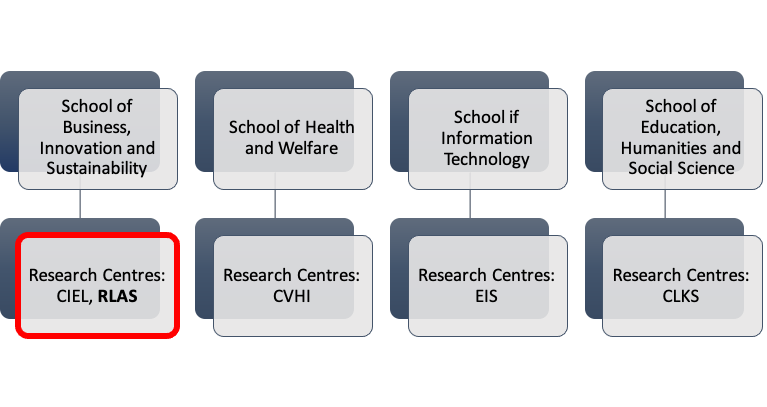
\includegraphics[width=12cm]{Pictures/SchoolsHH}
\caption[Organization chart of the Schools at Halmstad University]{Organization chart of the Schools at Halmstad University\cite{UniversityOrga}}
\label{Schools_HH}
\end{center}
\end{figure}

This is also shown as an organisational chart in figure \ref{Schools_HH} (see Appendix \ref{AppChart} for the full organisation chart). The Rydberg Laboratory for Applied Science is the largest and best established laboratory at Halmstad University. It consists of several small research laboratory units, conducting research in basic and applied science in areas such as mechanical engineering, nanotechnology, physics, chemistry, biomechanics, biomedicine, biology, environmental and energy science.\cite{RydbergCoreLab}\\
The Laboratory was opened in the year 2004 and was named after the famous Swedish physicist and mathematician Johannes "Janne" Rydberg. Johannes Rydberg was born in 1854 in Halmstad and is mainly known for the Rydberg formula, which is used to predict the wavelength of the spectral lines of the elements. He is often referred to as the Father of modern atomic spectroscopy.
 



%% Section 2 %%
\section{Presentation of clients}
\subsection{Volvo Cars}
Volvo Cars (see Appendix \ref{AppLoC}), latin for "I roll", is an international manufacturer of cars, known for products meeting the highest demands in security, quality and longevity. The company was founded by Assar Gabrielsson and Gustaf Larsson in 1927 in Gothenburg.\\
Some of the most important innovations in safety and sustainability, like the safety belt, the rear facing child seat and the lambda probe, were invented by Volvo Cars.\\
Nowadays Volvo Cars employs 43.000 employees and sells approximately 700.000 cars in over 100 different countries.\cite{VolvoCars}



%% Section 3 %%
\section{Project Background}
As mentioned previously, Halmstad University is cooperating with many different companies in the private sector. A big part of this is the car industry and particular the Volvo Car Group (VCG). In February of 2020, VCG proposed the measurement of transparent parts as a new research topic to the RLAS research center of Halmstad University. This was caused by the increasing use of transparent materials in both functional parts as well as in design parts as for example: integrated solar cells, adjustable tinting and integrated lights.\\
The transparent material project is driven by an attribute area of VCG called Perceived Quality Material Team. The project is an objective approach to measure visual appearance aspects such as colour and gloss on transparent materials. Its aim is to assist and maybe replace current measurement techniques used to define tolerance limits for transparent materials in Quality Control (QC).\\
The project was initially picked up at Halmstad University by the french student Romain Chanal and was continued with the beginning of this thesis. During his studies Chanal proposed a measurement method to the Perceived Quality Material Team. This measurement method was split into two, "hard metrology" and "soft metrology". The soft metrology part will determine the customer's tolerances regarding visual continuity of car bodies. It will be executed in a scientific study with a selected Group of people. As counterpart to that, the hard metrology part will be an optical measurement setup, representing the human visual perception. As final step these methods will be combined to an objective measurement method for car body parts in QC. Due to its similarity to the human eye and the human visual perception the measurement setup is referred to as "Artificial Eye" (AE).\cite{Chanal2020}
%TODO Introduction Add Picture with region of interest to Project Background (Car Picture Romain Report)

\subsection{Aim of Study}
The aim of this project is the setup, testing, qualification and optimisation of the optical measurement system "Artificial Eye". After the work of Romain Chanal, who came up with the basic layout of the optical system, the next step is its physical realisation. Further, the software for data acquisition, processing as well as control of the measurement setup needed to be developed. The control and processing software for the different components of the setup will be controlled via a Graphical User Interface (GUI). The final goal of this thesis is to complete phase one of the development process of the Artificial Eye, as shown in figure \ref{ChainIni}. Marked with a green border is the conceptional work finished by Romain Chanal. Marked with a red boarder are the remaining steps that will be discussed in this thesis.

\begin{figure}[h]
\begin{center}
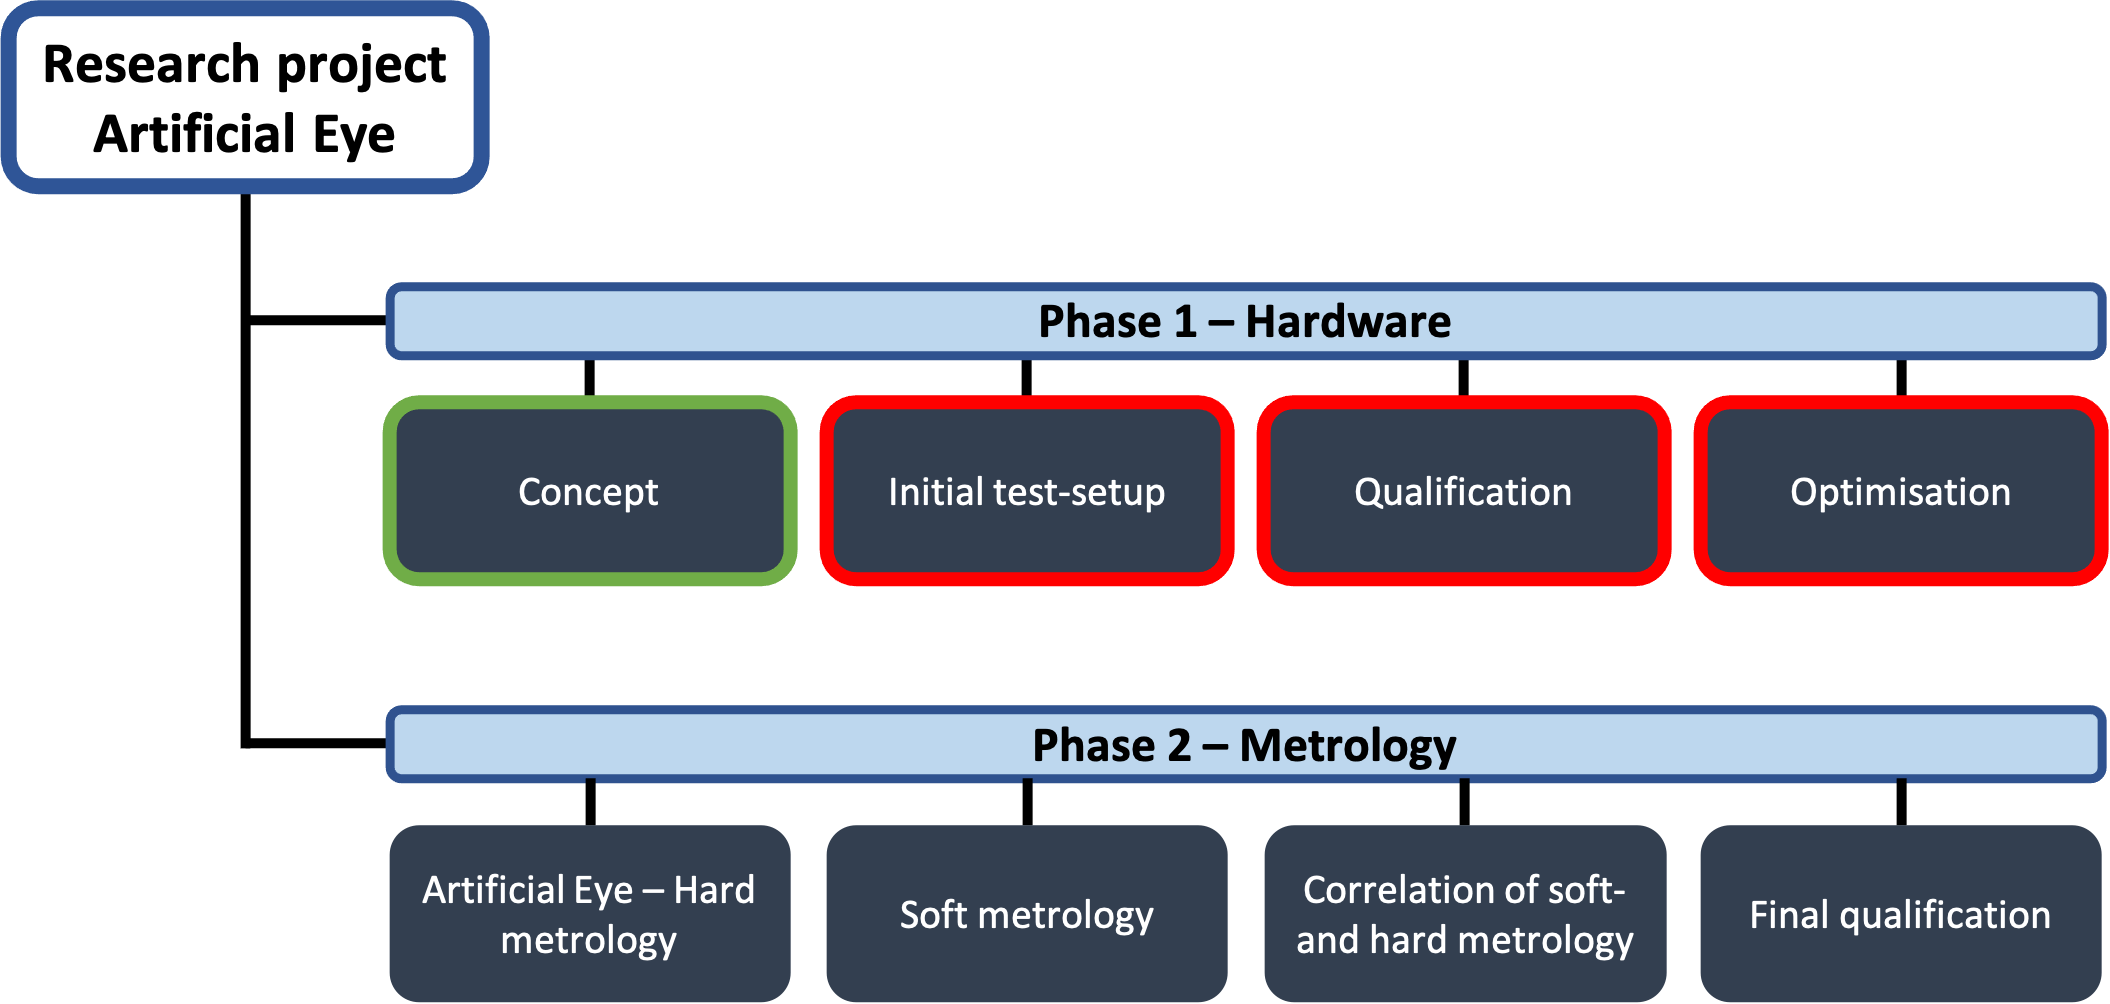
\includegraphics[width=12cm]{Pictures/ChainIntro}
\caption[Overview of the needed development steps]{Overview of the needed development steps: Green - Completed, Red - Open}
\label{ChainIni}
\end{center}
\end{figure}

\newpage
\subsection{Limitations}
In this thesis report, the work of Romain Chanal, who designed the basic layout of the optical system is continued.\\
This thesis is focussed only on the setup of the optical, mechanical and electrical part of the Artificial Eye. It will not include the scientific study of the human visual perception nor the combination of hard- and soft metrology. 






















